\label{chap:general_slam} 
\lettrine{T}he previous chapters described techniques for tracking robot arms in real-time using both external depth cameras, and depth cameras mounted on the robot arm itself. Though fast and efficient, these techniques are both essentially simple filters on the robot's state that make a strong \textit{Markov assumption}. That is, they assume that the current state of the robot can be derived entirely from the previous state of the robot and current sensor measurements. In the case of ARM-SLAM (the algorithm presented in chapter \ref{chap:dense_slam}), the algorithm suffers from drift in both the robot's state and the map because of this assumption. Further, these techniques only considered the joint angles of the robot as the state of the system, ignoring error from the extrinsic calibration of the sensor, motion of the base, or inaccuracies in the robot's model. Further, they made no attempt at modeleing the uncertainty of the robot state, and only predicted the maximum likelihood estimate of the state.

In this chapter, we will address these limitations by invoking a general graphical model that describes arm tracking and calibration. This model is able to support sensors of many kinds (even monocular sensors), and combines data from the joint encoders with data from the camera in a principled way. By making the model more general, we are able to add more degrees of freedom to the state (at some expense to performance).

\section{Problem Definition}
Consider the case of a monocular (\ie~2D) camera attached to a robot arm with inaccurate joint angle sensing. Suppose that the camera is attached in such a way that it can't see any part of the robot's body. As the robot moves around and collects data, how can we:

\begin{itemize}
  \item Predict the robot's joint angles over time?
  \item Create a consistent map of the scene?
  \item Find the extrinsic calibration of the sensor relative to the end effector?
  %\item Extract motion of the robot's base over time?
  \item Estimate the uncertainty in all of these unknown variables?
\end{itemize}

\noindent Formally, at a series of discrete timesteps $1, \ldots, T$, the robot receives synchronized monocular images $\Image_1, \ldots, \Image_T$ and joint encoder measurements of position $\enc_1, \ldots, \enc_T$ and velocity $\dot{\enc_t}, \ldots \dot{\enc_t}$. Unknown state variables of the system we wish to estimate include the robot's configuration $\qvec_1, \ldots, \qvec_T$, an unknown fixed extrinsic calibration $\Extr \in \SEThree$, and an unknown map $\SparseMap$, which we will represent as a series of discrete landmarks $\{\landmark_1, \ldots, \landmark_M\}$. 

\section{Graphical Model}
The problem can be represented as a graphical model with factors representing priors and measurement posteriors connecting nodes representing 3D landmarks, robot configurations, and camera extrinsics. \figref{fig:graphical_model} shows an example of the graphical model used.

\begin{figure}[width=1.0\textwidth]
\centering
\begin{tikzpicture}[x=2cm, y=2.0cm, every node/.style={scale=2.0}]
	\node[latent] (k0) {$\Extr$};
	\node[latent, below right = of k0] (q1) {$\config_1$};
	\node[latent, right=of q1] (q2) {$\config_2$};
	\node[latent, right=of q2] (qN) {$\config_{\ldots}$};
    \node[latent, right=of qN] (qT) {$\config_T$};
    \node[latent, above right=of k0] (l1) {$\landmark_1$};
    \node[latent, right=of l1] (lN) {$\landmark_{\ldots}$};
    \node[latent, right=of lN] (lM) {$\landmark_M$};
    \factor[below=of l1] {l1-f} {above right:$f_{\config_1, \landmark_1}$}{}{};
    \factor[below=of lN] {lN-f} {above right:$f_{\config_2, \landmark_{\ldots}}$}{}{};
    \factor[below=of lM] {lM-f} {above right:$f_{\config_{\ldots}, \landmark_M}$}{}{};
    \factor[below=of q1] {q1-f} {below:$f_{\enc_1}$}{}{};
    \factor[below=of q2] {q2-f} {below:$f_{\enc_2}$}{}{};
    \factor[below=of qN] {qN-f} {below:$f_{\enc_{\ldots}}$}{}{};
    \factor[below=of qT] {qT-f} {below:$f_{\enc_T}$}{}{};
    \factor[right=of q1] {q1q2-f} {below:$f_{\dot{\enc}_1}$}{}{};
    \factor[right=of q2] {q2qN-f} {below:$f_{\dot{\enc}_{\ldots}}$}{}{};
    \factor[right=of qN] {qNqT-f} {below:$f_{\dot{\enc}_{T - 1}}$}{}{};
    \factor[left=of k0]{k0-f}{below:$f_{\Extr}$}{}{};
    \factoredge{k0}{k0-f}{};
    \factoredge{q1}{q1-f}{};
	\factoredge{q2}{q2-f}{};
	\factoredge{qN}{qN-f}{};
	\factoredge{qT}{qT-f}{};
	\factoredge{q1}{q1q2-f}{};
    \factoredge{q2}{q1q2-f}{};
    \factoredge{qN}{q2qN-f}{};
    \factoredge{q2}{q2qN-f}{};
    \factoredge{qT}{qNqT-f}{};
    \factoredge{qN}{qNqT-f}{};
    \factoredge{q1}{l1-f}{};
    \factoredge{q2}{lN-f}{};
    \factoredge{qN}{lM-f}{};
    \factoredge{l1}{l1-f}{};
    \factoredge{lM}{lM-f}{};
    \factoredge{lN}{lN-f}{};
    \factoredge{k0}{l1-f}{};
    \factoredge{k0}{lN-f}{};
    \factoredge{k0}{lM-f}{};
\end{tikzpicture}
\caption{Graphical model of the SLAM system.}
\label{fig:graphical_model}
\end{figure}

Each time a camera at timestep $t$ observes landmark $i$, we have a factor $f_{\config_t, \landmark_i}$ that correlates together the cmaera calibration, robot configuration, and landmark position. For simplicity \figref{fig:graphical_model} shows only one landmark observation per timestep, but in fact there may be many landmarks observed. The joint encoders are connected to robot configurations by the factors $f_{\theta_t}$. Robot configurations are themselves correlated over time by the fators $f_{\dot{\enc}_{t-1}}$. 

In the coming sections, we will describe how each of these nodes and factors are expressed in practice.

\subsection{Landmark Observation Factors}

\begin{figure}
\centering
\begin{tikzpicture}
  	\node[anchor=south west,inner sep=0] (image) at (0,0) {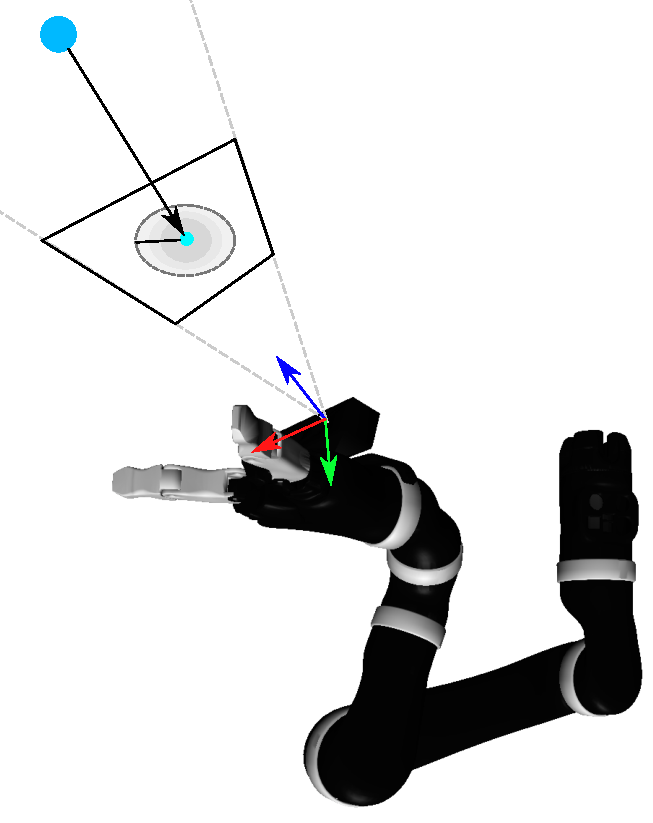
\includegraphics[width=0.75\textwidth]{img/graph_slam/projection_factor.pdf}};
  	\begin{scope}[x={(image.south east)},y={(image.north west)}]%
		%\draw[help lines,xstep=.1,ystep=.1] (0,0) grid (1,1); 
	    %\foreach \x in {0,1,...,9} { \node [anchor=north] at (\x/10,0) {0.\x}; }
	    %\foreach \y in {0,1,...,9} { \node [anchor=east] at (0,\y/10) {0.\y}; }
	    \node at (0.31, 0.69) {\Large$\measurement_i$};
	    \node at (0.1, 0.9) {\Large$\landmark_i$};
	    \node at (0.26, 0.685) {\Large$\Sigma_{\measurement}$};
	    \node at (0.55, 0.55) {\Large$\Extr$};
	    \node at (0.41, 0.78) {\Large$\Image_t$};
	    \node at (0.2, 0.2) {\Large$\config_t \left\{ \rule{0pt}{20mm}\right.$};
    \end{scope} 
\end{tikzpicture} 
\caption{Landmark observation factor. The robot at configuration $\config_t$ observes landmark $\landmark_i$ in image $\Image_t$. The noise is on the reprojection of the landmark into the image.}
\end{figure} 

The factors $f_{\config_t, \landmark_i}$ of the graph (\figref{fig:graphical_model}) represent the posterior probability of the robot's configuration, camera extrinsics, and landmark position given observations of the landmark $i$ at time $t$.

\begin{equation} 
	f_{\config_t, \landmark_i} = \Prob\left( \measurement_{i, t} | \config_t, \landmark_i, \Extr\right)
\end{equation}

\noindent here, we model a measurement of landmark $\landmark_i$ in camera image $I_t$ as a 2D pixel coordinate $\measurement_{i, t}$. The 3D landmark positions $\landmark_i$ is projected onto the camera image using the projection function

\begin{equation}
	 F_{\Proj}\left(\config_t, \Extr, \landmark_i\right) = \Proj\left(\left(F(\config) \Extr \right)\inv\landmark_i\right) 
\end{equation}

\noindent the measurement $\measurement_{i, t}$ can be modeled as a random variable sampled from the distribution

\begin{equation}
	\measurement_{i, t} \sim F_{\Proj}\left(\config_t, \Extr, \landmark_i\right) + \mathcal{N}(\mu_\measurement, \Sigma_\measurement)
\end{equation}

\noindent where $\mu_\measurement, \Sigma_\measurement$ are the mean and variance of the reprojection noise, respectively. Therefore,

\begin{equation}
	\Prob\left( \measurement_{i, t} | \config_t, \landmark_i, \Extr\right) = \mathcal{N}_{\mu_\measurement, \Sigma_\measurement}\left(F_{\Proj}\left(\config_t, \Extr, \landmark_i\right) - \measurement_{i, t}\right)
\end{equation}

\subsection{Joint Encoder Factors}
The factors $f_{\enc_t}$ represent the posterior probability of the robot's configuration given the joint encoder measurements at time $t$. That is

\begin{equation}
	f_{\enc_t} = \Prob\left(\enc_t | \config_t\right)
\end{equation}

\noindent as in chapters \ref{chap:dense_external_tracking} and \ref{chap:dense_slam}, we assume that the joint encoders are random variables drawn from gaussian noise on the true configuration of the robot

\begin{equation}
	\enc_t \sim K_\enc\inv\left(\config_t + \mathcal{N}(\mu_\enc, \Sigma_\enc)\right)
\end{equation}

\noindent where $\mu_\enc, \Sigma_\enc$ are the mean and covariance of the joint angle noise, respectively, and $K_\enc$ is the static joint encoder calibration function (\sref{sec:encoders}). Therefore the posterior is

\begin{equation}
	\Prob\left(\enc_t | \config_t\right) = \mathcal{N}_{\mu_\enc, \Sigma_\enc}\left(\config_t - K_\enc(\enc_t)\right)
\end{equation}

To account for gear backlash (\sref{sec:encoders}), we add a small \textit{dead band} $\Delta_\enc$ so that configurations within $\Delta_\enc$ of the joint encoders are not penalized:

 \begin{align}
	\Prob\left(\enc_t | \config_t\right) &= \mathcal{N}_{\mu_\enc, \Sigma_\enc}\left(\delta(\config_t - K_\enc(\enc_t))\right) \\
	\delta(\config_t - K_\enc(\enc_t)) &= \colvec{3}{\max\left\big(0, \|\config_t[1] - K_\enc(\enc_t)[1]\| - \Delta_\enc\right\big)\text{sgn}\left(\config_t[1] - K_\enc(\enc_t)[1]\right)}{\vdots}{\max\left\big(0, \|\config_t[N] - K_\enc(\enc_t)[N]\| - \Delta_\enc\right\big)\text{sgn}\left(\config_t[N] - K_\enc(\enc_t)[N]\right)}
\end{align}

\noindent where $\text{sgn}$ is the sign function. The gear backlash term $\delta$ allows the joint angles of the robot to vary within the dead-band $\Delta_\enc$ without penalty.

\subsection{Robot Dynamics Factors}

The factors $f_{\dot{\enc}_{t- 1}}$ correlate the robot's joint angles given joint velocity measurements $\dot{\enc}_{t - 1}$. That is

\begin{equation}
	f_{\dot{\enc}_{t- 1}} = \Prob(\dot{\enc}_{t - 1} | \config_{t - 1}, \config_{t})
\end{equation}

\noindent we assume that the velocity measurements are random variables drawn from the true velocity of the robot's joints, which we approximate with finite differencing. That is

\begin{equation}
	\dot{\enc}_{t - 1} \sim \frac{\qvec_{t} - \qvec_{t - 1}}{\Delta t} + \mathcal{N}(\mu_{\dot{\theta}}, \Sigma_{\dot{\theta}})
\end{equation}

\noindent where $\delta t$ is the timestep between time $t$ and $t-1$, $\mu_{\dot{theta}}$ is the mean of the velocity noise, and $\Sigma_{\dot{\theta}}$ is its covariance. Therefore

\begin{equation}
	\Prob(\dot{\enc}_{t - 1} | \config_{t - 1}, \config_{t}) = \mathcal{N}_{\mu_{\dot{\theta}}, \Sigma_{\dot{\theta}}}\left(\dot{\enc}_{t - 1} - \frac{\qvec_{t} - \qvec_{t - 1}}{\Delta t}\right)
\end{equation} 

The dynamics factors smooth our estimate of the joint angle trajectory so that it is closer to physically feasible than if only joint encoder factors are used. In part, we do this because the joint encoder posterior is not really representative of the true system dynamics that cause the joint encoders to be inaccurate. The inaccuracy stems from unmodeled systematic error that depends in part on the robot's configuration and torques it is applying. Adding a factor to constrain the motion of the joints allows us to smoothly predict the joint encoder error without having to explicitly model the physical process that causes it.

\subsection{Extrinsic Prior}
The factor $f_{\Extr}$ describes the prior distribution for the camera extrinsics. This is simply

\begin{align}
	f_{\Extr} &= \Prob(\Extr) \\
		      &= \mathcal{N}_{\mu_{\Extr}, \Sigma_{\Extr}}(\Extr)
\end{align}

\noindent where $\mu_{\Extr}, \Sigma_{\Extr}$ are the mean and covariance of the extrinsic prior, respectively.

\section{SLAM Back-end System Implementation}
As the robot receives joint encoder measurements and observations of landmarks, we add nodes and factors to the graphical model, which is then jointly optimized to find a maximum likelihood estimate of all the unknown variables ($\config_1, \ldots \config_T$, $\landmark_1, \ldots, \landmark_M$ and $\Extr$) given all the measurements. We consider both batch and online solutions. 

For the batch solution, we use Levenberg-Marquadt. For the online solution, we use the Incremental Smoothing and Mapping 2 (iSAM2) algorithm \cite{Kaess12ijrr}. For an explanation of how these algorithms work, \sref{sec:graph_slam}. We use off-the-shelf implementations of these algorithms from the Georgia Tech Smoothing and Mapping (GTSAM) \cite{gtsam} library, and make use of the outlier-robust Cauchy estimator found in GTSAM. 

\section{Landmark Front-end System Implementation}
To acquire landmarks from the camera images, we consider two systems: one based on April \cite{olson2010tags} tags, and another based on natural image features using the Binary Robust Invariant Scalable Keypoint (BRISK)\cite{Leutenegger2011BRISK} features.

\subsection{April Tag Front-end Implementation}

April tags are fiducials designed for computer vision and augmented reality consisting of unique grid patterns. These tags can be detected easily in 2D images, and with a known intrinsic calibration and tag size, their poses relative to the sensor can be estimated. Using April tags, the landmark $\landmark_i$ is simply the 3D location of the top-left corner of the April tag with tag id $i$. The initial position estimate of $\landmark_i$ is given by the pose estimate returned by the April tags detector (which also reports the pixel locations of each of the tag's corners). 

\begin{figure}
	\centering
	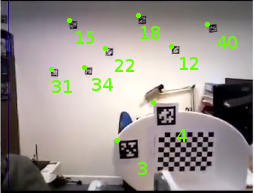
\includegraphics[width=0.5\textwidth]{img/graph_slam/apriltags}
	\caption{Detected April tags and their associated IDs.}
	\label{fig:april_tags}
\end{figure}

The April tags were used mainly to test the SLAM backend system without having to worrry about landmark association. Our system does not require the tags to detect and associate landmarks, but will use them when available.

\subsection{Natural Image Feature Front-end Implementation}

Acquiring and associating 3D landmarks from a series of natural images is somewhat more complicated than acquiring 3D landmarks from fiducials. First, we acquire a number of BRISK keypoints (\sref{sec:image_features}) $k_1, \ldots, k_n$ in the image $\Image_t$ roughly corresponding to corners and lines. Each keypoint is associated with a descriptor $d_1, \ldots, d_n$. 

\begin{figure}
	\centering
	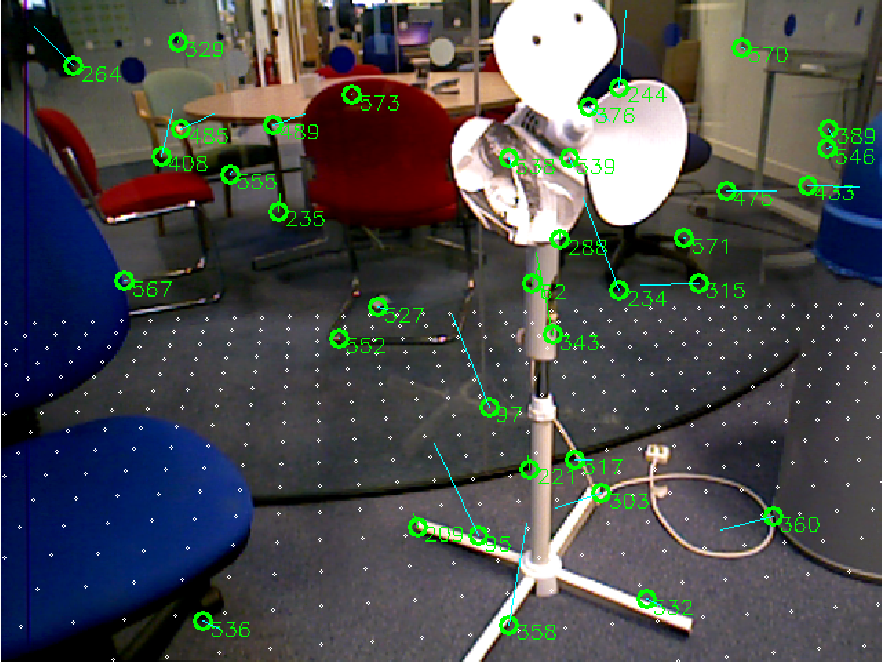
\includegraphics[width=0.5\textwidth]{img/graph_slam/brisk_features}
	\caption{Detected BRISK keypoints (green circles), their IDs, and reprojection error (blue lines). Also shown is the predicted ground plane (grey dots).}
	\label{fig:brisk_detections}
\end{figure}

Then, for each keypoint, we match it to the closest potential 3D landmark visible from the estimated robot configuration $\config_t$. We reject the match whenever the descriptor $d_i$'s Hamming distance to the existing landmark's last observed descriptor is too far, and accept it otherwise. Rejected matches get added to the pool of new potential 3D landmarks, but are not added to the facor graph until the following conditions are met:

\begin{itemize}
  \item The landmark has been matched to two or more camera images.
  \item There is a sufficient stereo baseline between camera observations of the landmark.
  \item The landmark can be successfully stereo-triangulated (\sref{sec:triangulation}) from its observations.
\end{itemize} 

The stereo triangulation system uses the current estimate of the robot's configuration to estimate the motion between frames. By conservatively eliminating outliers in this way, we minimize false-positive associations between image features. Still, some false-positive associations occur.

\section{Experiments}